\section{Hardware Setup}
\subsection{Circuit Design}
% The evaluation circuit is primarily composed of three AD8421 instrumentation amplifiers \cite{ad8421_datasheet} and one ADA4522 operational amplifier \cite{ada4522_datasheet}. To facilitate a systematic analysis, the circuit can be divided into distinct functional partitions.

% \subsection{System Architecture Overview}

The hardware front-end for the impedance spectroscopy measurement system is designed to generate a precisely conditioned excitation signal, apply it to the target load, and capture the resulting differential voltage and current. To facilitate a clear understanding of the signal flow, the circuit is logically partitioned into five sequential stages, which is also depicted here in \ref{fig:overal-circuit}:

\begin{figure}[h!]
    \centering
    
\includegraphics[width=1\textwidth]{New_circuit.png}
    \caption{Overal circuit in LTSpice}
    \footnotemark
    \label{fig:overal-circuit}
\end{figure}


\begin{enumerate}
    \item \textbf{Stage 1: DC Reference Generation:} The system begins by establishing a highly stable 1.65V DC reference voltage. This bias is derived from the main 5V supply and buffered to provide a low-impedance foundation. This ensures that the single-supply Analog-to-Digital Converters (ADCs) and instrumentation amplifiers can operate around a centered, virtual ground.
    
    \item \textbf{Stage 2: Signal Conditioning (DAC Output):} A unipolar multisine excitation signal (ranging from 0.0V to 3.3V) is generated by the STM32 microcontroller. This stage utilizes an instrumentation amplifier to subtract the 1.65V reference from the source, effectively level-shifting the waveform into a bipolar AC signal (-1.65V to +1.65V). This critical step prevents DC polarization of the target load.
    
    \item \textbf{Stage 3: The Device Under Test (DUT):} The conditioned AC signal is driven into the measurement path. This physical path consists of the target impedance network (the DUT) connected in series with a known precision shunt resistor to ground. 
    
    \item \textbf{Stage 4: Differential Voltage Measurement ($U_v$):} A dedicated instrumentation amplifier is positioned directly across the DUT to measure the precise voltage drop. This differential AC signal is captured and level-shifted back to a 1.65V DC center to match the unipolar input requirements of the microcontroller's ADC.
    
    \item \textbf{Stage 5: Current Measurement ($U_i$):} A parallel instrumentation amplifier measures the voltage drop across the series shunt resistor. Because the shunt resistance is a known constant, this voltage is directly proportional to the current flowing through the DUT. Like the voltage measurement, this signal is level-shifted and filtered before being routed to the ADC.
\end{enumerate}

By capturing both the $U_v$ and $U_i$ signals simultaneously through these five stages, the microcontroller can perform discrete Fourier transforms // Goertez algorithm on the synchronized data to calculate the complex impedance of the DUT across the generated frequency spectrum.

\subsubsection{Stable 1.65V Reference Supply}\label{sec:1.65}
% A stable 1.65\,V reference voltage is required to bias the Digital-to-Analog Converter (DAC) and Analog-to-Digital Converter (ADC) components without introducing drift. This is achieved using a voltage divider network connected to a stable 5\,V source. The divider consists of a 6.7\,k$\Omega$ and a 3.3\,k$\Omega$ resistor, scaling the voltage appropriately:

% \begin{equation}
%     V_{ref} = 5\,\text{V} \times \frac{3.3\,\text{k}\Omega}{6.7\,\text{k}\Omega + 3.3\,\text{k}\Omega} = 1.65\,\text{V}
% \end{equation}

% The scaled voltage is subsequently filtered through a 10\,$\mu$F capacitor to attenuate high-frequency noise. Finally, the signal is buffered using an ADA4522 operational amplifier configured as a voltage follower. This configuration provides a low-impedance output for the 1.65\,V reference, ensuring stability under varying load conditions from the downstream components \cite{ada4522_datasheet}.

A stable reference voltage (nominally 1.65\,V) is required to bias the Digital-to-Analog Converter (DAC) and Analog-to-Digital Converter (ADC) components without introducing drift. This is achieved using a voltage divider network connected to a stable 5\,V source. To improve power supply rejection and ensure stability, the 5\,V source is initially decoupled with a $1\,\mu\mathrm{F}$ capacitor (C3).

The voltage divider itself consists of a $680\,\Omega$ resistor ($R_8$) and a $330\,\Omega$ resistor ($R_9$), which scales the voltage according to the standard voltage divider formula:
\begin{equation}
    V_{ref} = 5\,\mathrm{V} \times \frac{330\,\Omega}{680\,\Omega + 330\,\Omega} \approx 1.634\,\mathrm{V}
\end{equation}

This scaled voltage, which provides an effective nominal center point for the $3.3\,\mathrm{V}$ ADC logic, is subsequently filtered through a $10\,\mu\mathrm{F}$ capacitor (C2) to attenuate high-frequency noise. Finally, the signal is buffered using an ADA4522-1 operational amplifier (U6) configured as a voltage follower. This configuration provides a low-impedance output for the reference voltage, ensuring stability under varying load conditions from the downstream components \cite{ada4522_datasheet}.

\subsubsection{The DAC Output Stage}

The DAC partition utilizes an AD8421 instrumentation amplifier (U4) to condition the multisine signal generated by the STM32 microcontroller. The AD8421 is selected for its high common-mode rejection and differential input configuration \cite{ad8421_datasheet}. 

The STM32 generates a unipolar multisine signal ($V_{dac}$) ranging from 0.0\,V to 3.3\,V. To prevent DC polarization in the subsequent ADC stage and the Device Under Test (DUT), this signal must be centered around zero. The AD8421 achieves this by subtracting the buffered reference voltage, mentioned in \textbf{Sec.}\ref{sec:1.65}, from the source signal. 

To appropriately scale the output, this stage utilizes a gain resistor ($R_7$) of $100\,\mathrm{k}\Omega$ connected across the RG pins. According to the AD8421 datasheet \cite{ad8421_datasheet}, the gain $G$ is determined by the equation $G = 1 + \frac{9.9\,\mathrm{k}\Omega}{R_G}$, resulting in a nominal gain of approximately $1.099$.

The general transfer function for the AD8421 is explicitly defined in its datasheet as \cite{ad8421_datasheet}:
\begin{equation}
    V_{OUT} = G \times (V_{+IN} - V_{-IN}) + V_{REF}
\end{equation}

In this circuit configuration, the multisine signal is fed into the non-inverting input ($V_{+IN} = V_{dac}$), the stable reference voltage is connected to the inverting input ($V_{-IN} \approx 1.634\,\mathrm{V}$), and the output reference pin is tied directly to ground ($V_{REF} = 0\,\mathrm{V}$). Substituting these parameters yields the specific output equation:
\begin{equation}
    V_{OUT} = 1.099 \times (V_{dac} - 1.634\,\mathrm{V})
\end{equation}

This mathematical shift effectively translates and slightly amplifies the original unipolar signal into a bipolar AC waveform. 

The physical pin configuration of the AD8421 in this setup is illustrated in Figure \ref{fig:ad8421_pinout} and detailed as follows:
\begin{itemize}
    \item \textbf{Pin 1 (-IN):} Connected to the stable reference supply from U6.
    \item \textbf{Pins 2 \& 3 (RG):} Connected to the $100\,\mathrm{k}\Omega$ gain resistor ($R_7$).
    \item \textbf{Pin 4 (+IN):} Connected to the multisine signal input from the STM32.
    \item \textbf{Pin 5 (-VS):} Connected to the $-5$\,V power supply.
    \item \textbf{Pin 6 (REF):} Connected to system ground (GND).
    \item \textbf{Pin 7 (VOUT):} The conditioned output signal, passed to the DUT.
    \item \textbf{Pin 8 (+VS):} Connected to the $+5$\,V power supply.
\end{itemize}

\begin{figure}[h!]
    \centering
    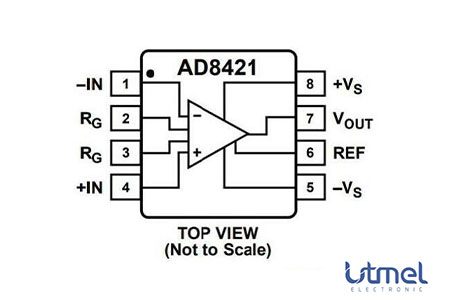
\includegraphics[width=0.6\textwidth]{AD8421.jpg}
    \caption{Pin layout and configuration of the AD8421}
    \footnotemark
    \label{fig:ad8421_pinout}
\end{figure}
\footnotetext{Source: \url{https://www.utmel.com/components/ad8421-amplifier-pinout-datasheet-schematic?id=745}}

% ##############################################################

% The DAC partition utilizes an AD8421 instrumentation amplifier to condition the multisine signal generated by the STM32 microcontroller. The AD8421 is selected for its high common-mode rejection and differential output configuration \cite{ad8421_datasheet}. 

% The AD8421 achieves this by subtracting the 1.65\,V reference from the source signal. The general transfer function for the AD8421 is given by the following equation:
% \begin{equation}
%     V_{OUT} = G \times (V_{+IN} - V_{-IN}) + V_{REF}
% \end{equation}

% By leaving the gain-setting pins (RG) unconnected, the amplifier gain $G$ is set to unity ($G = 1$). The circuit is configured such that the multisine signal is fed into the non-inverting input ($V_{+IN} = V_{dac}$), the stable reference voltage is connected to the inverting input ($V_{-IN} = 1.65\,\text{V}$), and the output reference pin is tied to ground ($V_{REF} = 0\,\text{V}$). Substituting these parameters into the transfer function yields:
% \begin{equation}
%     V_{OUT} = 1 \times (V_{dac} - 1.65\,\text{V}) + 0\,\text{V} = V_{dac} - 1.65\,\text{V}
% \end{equation}

% This mathematical shift effectively translates the original $0.0$\,V to $3.3$\,V unipolar signal into a bipolar signal with an output range of $-1.65$\,V to $+1.65$\,V.

% The STM32 generates a unipolar multisine signal ranging from 0.0\,V to 3.3\,V. To prevent polarization in the subsequent ADC stage and the Device Under Test (DUT), this signal must be centered around zero. The AD8421 achieves this by subtracting the 1.65\,V reference from the source signal. Specifically, the multisine signal is fed into the non-inverting input (IN+), while the stable 1.65\,V reference is connected to the inverting input (IN-). This effectively shifts the output signal range to $-1.65$\,V to $+1.65$\,V.

% The physical pin configuration of the AD8421 in this setup is illustrated in Figure \ref{fig:ad8421_pinout} and detailed as follows:
% \begin{itemize}
%     \item \textbf{Pin 1 (-IN):} Connected to the stable 1.65\,V reference supply.
%     \item \textbf{Pins 2 \& 3 (RG):} Left unconnected to set the amplifier gain to unity ($G = 1$).
%     \item \textbf{Pin 4 (+IN):} Connected to the multisine signal input from the STM32.
%     \item \textbf{Pin 5 (-VS):} Connected to the $-5$\,V power supply.
%     \item \textbf{Pin 6 (REF):} Connected to system ground (GND).
%     \item \textbf{Pin 7 (VOUT):} The conditioned output signal, passed to the DUT.
%     \item \textbf{Pin 8 (+VS):} Connected to the $+5$\,V power supply.
% \end{itemize}

% \begin{figure}[h!]
%     \centering
%     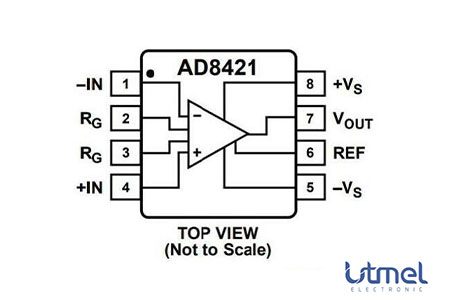
\includegraphics[width=0.6\textwidth]{AD8421.jpg}
%     \caption{Pin layout and configuration of the AD8421}
%     \footnotemark
%     \label{fig:ad8421_pinout}
% \end{figure}
% \footnotetext{Source: \url{https://www.utmel.com/components/ad8421-amplifier-pinout-datasheet-schematic?id=745}}


% The resulting level-shifted multisine waveform from the DAC stage is depicted in Figure \ref{fig:dac_output}. The oscilloscope captures two distinct traces: the prominent yellow trace represents the original multisine input signal generated by the STM32, while the fainter pink trace beneath it displays the conditioned output from the AD8421. 

% As observed in the figure, the output waveform successfully tracks the input with minimal visible noise. However, to further guarantee system stability and limit the effective bandwidth, the AD8421 datasheet suggests introducing a small capacitor into the configuration. Specifically, a $12\,\mathrm{pF}$ capacitor is recommended as a practical starting point to mitigate potential high-frequency instability under varying load conditions \cite{ad8421_datasheet}.

% \begin{figure}[h!]
%     \centering
%     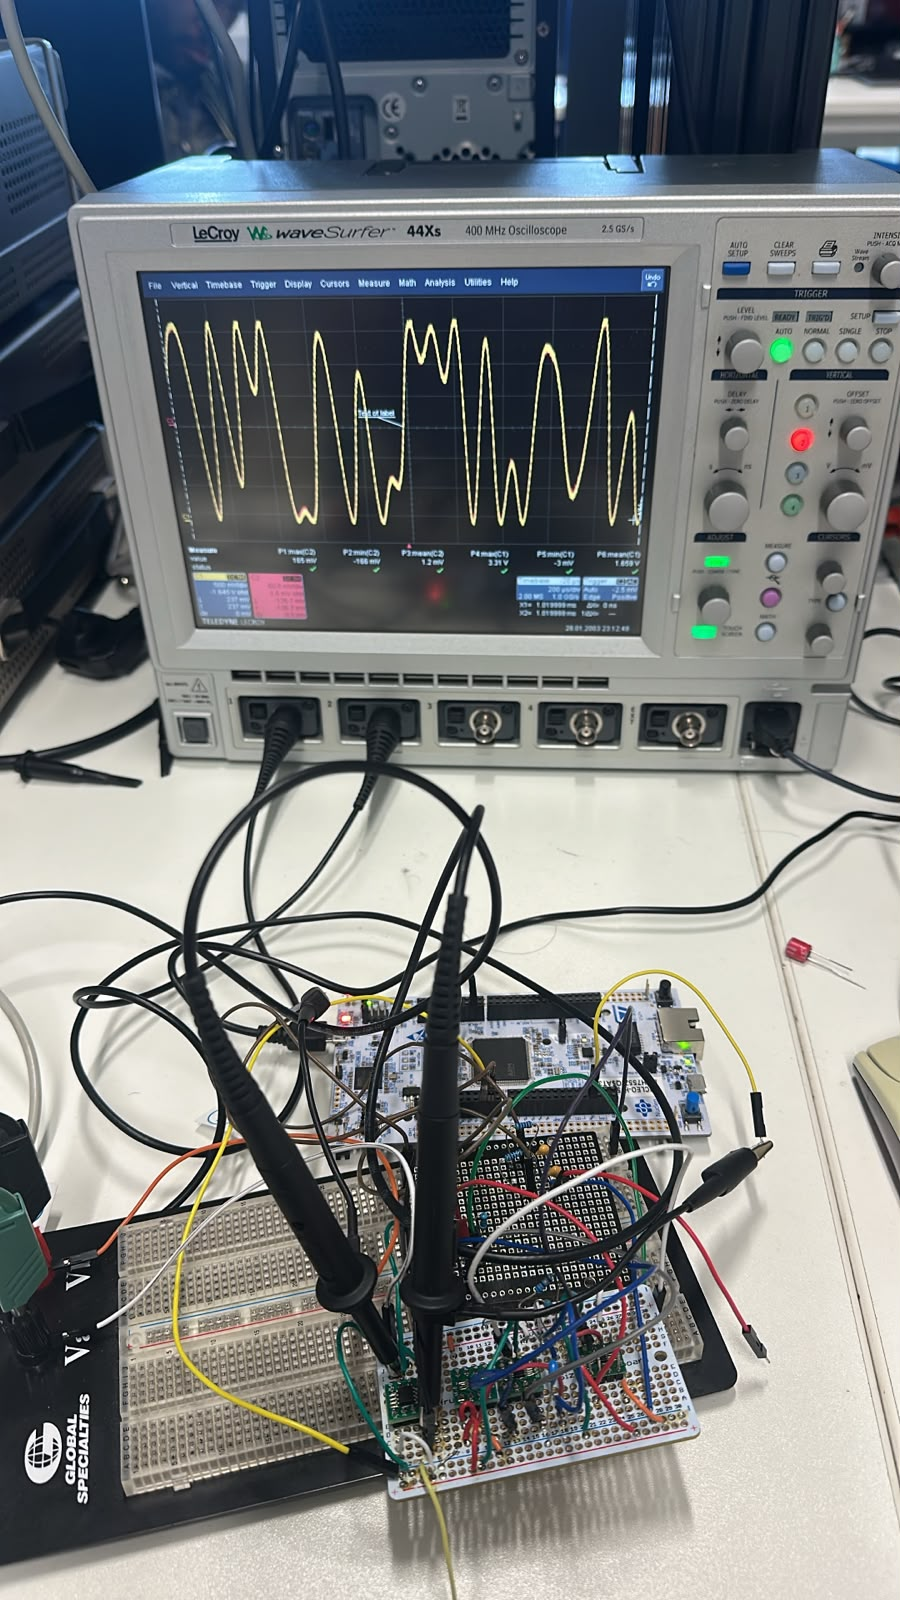
\includegraphics[width=0.5\textwidth]{dac_output.jpeg}
%     \caption{Output waveform of the DAC stage after level shifting via the AD8421.}
%     \label{fig:dac_output}
% \end{figure}
% ##############################################################
% \subsubsection{The DUT}
% The first Device under Test is a 1.5kOhm resistor connected in series with a parallel 4.7nF capacitor and a 1.5kOhm resistor. Another shunt resistor is then connected with the DUT in order to measure the current of the DUT. The output signal of the DAC is then passed to the DUT and the voltage and current are then measured and pass through the ADC component for further analysis.

\subsubsection{The Device Under Test (DUT)}
% To evaluate the measurement system, a known passive component network is utilized as the first Device Under Test (DUT). This network is modeled to represent a typical impedance load and consists of a $1.5\,\mathrm{k}\Omega$ resistor connected in series with a parallel combination of a $47\,\mathrm{nF}$ capacitor and a second $1.5\,\mathrm{k}\Omega$ resistor. 

% To enable current measurement, a $1.5\,\mathrm{k}\Omega$ shunt resistor ($R_{shunt}$) is connected in series with the DUT and tied to ground. When the conditioned multisine signal from the DAC stage is applied to the DUT, the resulting voltage across the DUT and the current flowing through the shunt resistor can be simultaneously captured for impedance spectroscopy analysis.

\subsubsection{The ADC Front-End (Signal Measurement)}
To accurately capture the voltage and current for the microcontroller's Analog-to-Digital Converter (ADC), the measurement stage employs two AD8421 instrumentation amplifiers. These amplifiers provide the necessary high common-mode rejection, low noise, and precise differential sensing required for reliable impedance calculations \cite{ad8421_datasheet}.

\begin{itemize}
    \item \textbf{Voltage Measurement ($U_v$):} The first AD8421 (U1) is configured to measure the differential voltage directly across the DUT. The non-inverting input (+IN) is connected to the node between the DUT and the shunt resistor, while the inverting input (-IN) is connected to the node preceding the DUT. 
    \item \textbf{Current Measurement ($U_i$):} The second AD8421 (U2) is dedicated to current measurement by capturing the voltage drop across the $1.5\,\mathrm{k}\Omega$ shunt resistor. Its non-inverting input (+IN) is tied directly to system ground (GND), and its inverting input (-IN) is connected to the node between the DUT and the shunt resistor.
\end{itemize}

Both amplifiers utilize a gain resistor ($R_G$) of $100\,\mathrm{k}\Omega$. According to the AD8421 transfer function ($G = 1 + 9.9\,\mathrm{k}\Omega / R_G$), this results in a nominal gain of approximately $1.099$. 

Furthermore, to ensure the measured bipolar signals are compatible with the unipolar $0.0\,\mathrm{V}$ to $3.3\,\mathrm{V}$ input range of the STM32's ADC, the reference pins (REF) of both AD8421 amplifiers are tied to the stable $1.65\,\mathrm{V}$ supply described in the previous section. This effectively level-shifts the $U_v$ and $U_i$ AC outputs to a $1.65\,\mathrm{V}$ DC center point.

Finally, in accordance with the manufacturer's recommendations for driving ADCs, the high-bandwidth outputs of the AD8421s should be routed through an RC low-pass filter before reaching the ADC pins. As noted in the component specifications, this filtering isolates the amplifier from the dynamic capacitive loading of the ADC inputs, reduces the effective noise bandwidth, and provides overload protection \cite{ad8421_datasheet}.

% \subsubsection{The ADC Stage}
% % Add your ADC documentation here
% The ADC consisits of 2 INA (AD8421) 

\subsection{Microcontroller and Digital Signal Processing}
The central processing and control unit of the measurement system is the STM32H755ZI-Q microcontroller, housed on a Nucleo-144 development board \cite{stm32_nucleo}.

To ensure strict timing deterministic behavior—which is critical for accurate phase measurements in impedance spectroscopy—the firmware heavily leverages hardware timers and Direct Memory Access (DMA). The code flow correlates directly to the hardware partitions as follows:

\begin{itemize}
    \item \textbf{Signal Generation (DAC \& DMA):} A 4096-point multisine waveform is pre-calculated and stored in the microcontroller's memory. Timer 4 (TIM4) is configured to trigger the Digital-to-Analog Converter (DAC1), while a DMA channel continuously streams the waveform array to the DAC register. This allows the STM32 to output the unipolar excitation signal to the hardware subtractor stage continuously without utilizing CPU cycles. In \textbf{Fig.}\ref{fig:DAC_output}, the multisine wave is measured using the oscilloscope
    
    
    \item \textbf{Simultaneous Acquisition (ADCs \& DMA):} The differential voltage ($U_v$) and current ($U_i$) signals conditioned by the AD8421 front-end are routed to two separate Analog-to-Digital Converters (ADC1 and ADC2). Timer 2 (TIM2) synchronizes both ADCs to sample at the exact same frequency. Two dedicated DMA streams capture 4096 samples into parallel memory buffers (\inlinecode{AdcBuffer1} and \inlinecode{AdcBuffer2}).
    
    \item \textbf{Interrupt and DSP Execution:} Once the DMA completes filling the 4096-point buffers, a hardware interrupt (\inlinecode{HAL\_ADC\_ConvCpltCallback}) sets a completion flag. The main loop halts the acquisition timer and begins processing the buffers. Using the CMSIS-DSP library, the firmware applies the Goertzel algorithm (or alternatively, a Fast Fourier Transform) to the sampled data. This extracts the precise magnitude and phase shift for the specific frequency bins present in the multisine signal.
    
    \item \textbf{Data Transmission:} After calculating the accumulated phase and magnitude, the results are formatted and transmitted via USART3 to a connected PC for final logging and visualization. 
\end{itemize}

\begin{figure}[h!]
        \centering
        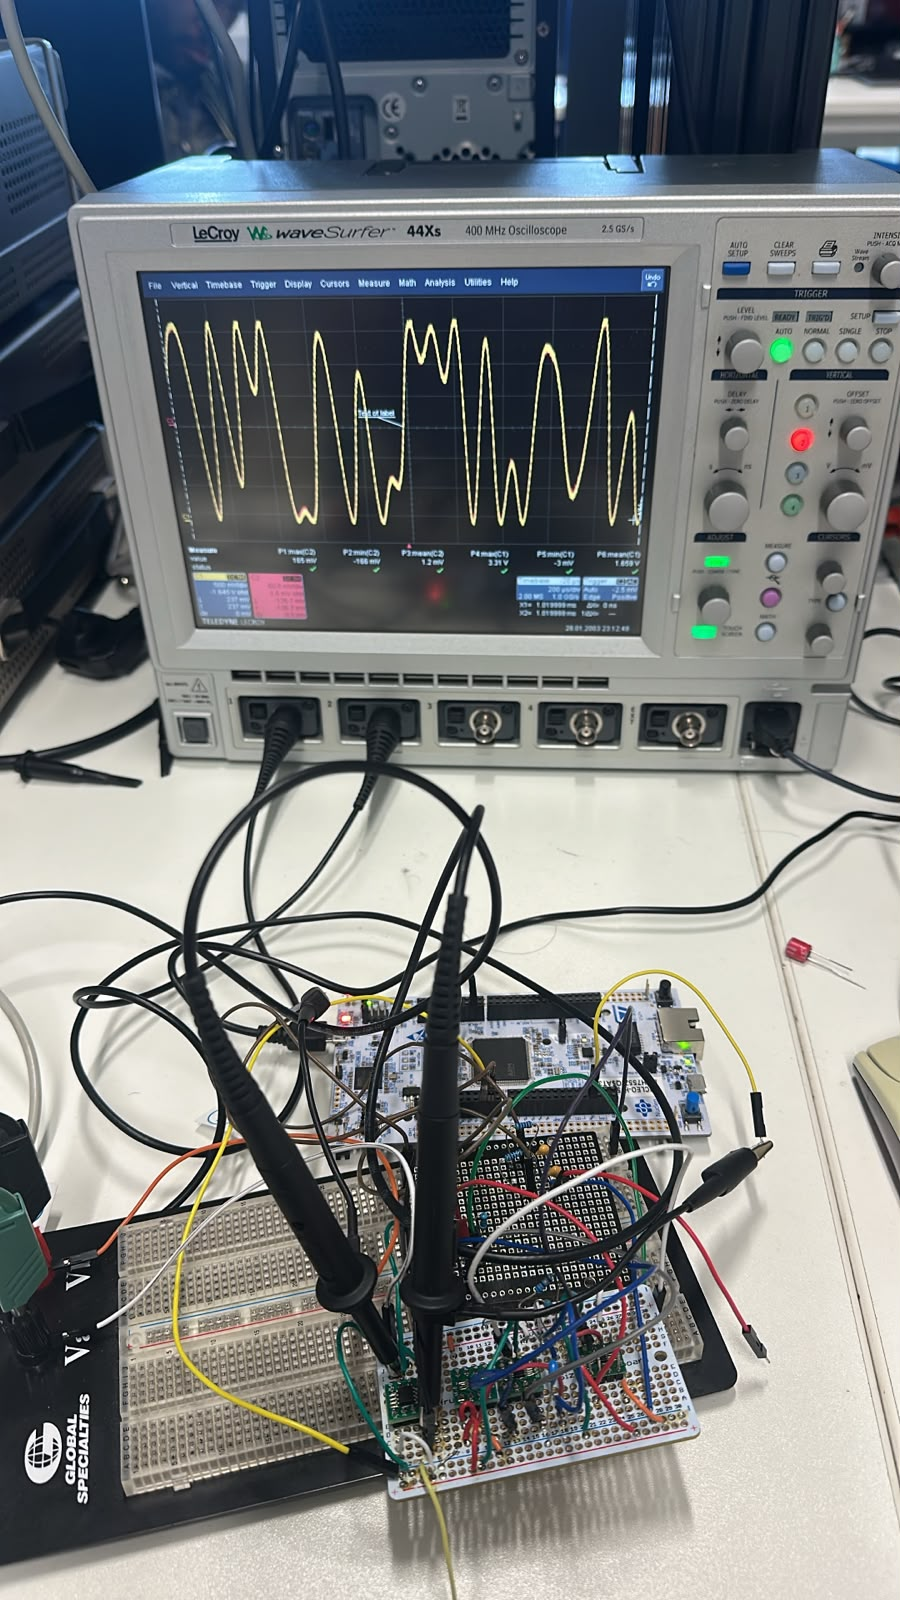
\includegraphics[width=1\textwidth]{dac_output.jpeg}
        \caption{DAC output from STM32 measured by oscilloscope}
        \footnotemark
        \label{fig:DAC_output}
    \end{figure}

\subsubsection{Firmware Execution Flow}
The sequential logic of the firmware, from peripheral initialization to the continuous DSP loop, is illustrated in Figure \ref{fig:stm32_flow_chart}.

\begin{figure}[h!]
    \centering
    
\includegraphics[width=0.8\textwidth]{Diagram_project.png}
    \label{fig:stm32_flow_chart}
    \caption{STM32 execution flow chart}
\end{figure}

\subsection{Setup}